\documentclass[12pt]{article}

%packages
%\usepackage{latexsym}
\usepackage{graphicx}
\usepackage{color}
\usepackage{amsmath}
\usepackage{dsfont}
\usepackage{placeins}
\usepackage{amssymb}
\usepackage{wasysym}
\usepackage{abstract}
\usepackage{hyperref}
\usepackage{etoolbox}
\usepackage{datetime}
\usepackage{xcolor}
\usepackage{alphalph}
\usepackage{fancyvrb}
\settimeformat{ampmtime}

%\usepackage{pstricks,pst-node,pst-tree}

%\usepackage{algpseudocode}
%\usepackage{amsthm}
%\usepackage{hyperref}
%\usepackage{mathrsfs}
%\usepackage{amsfonts}
%\usepackage{bbding}
%\usepackage{listings}
%\usepackage{appendix}
\usepackage[margin=0.9in]{geometry}
%\geometry{papersize={8.5in,11in},total={6.5in,9in}}
%\usepackage{cancel}
%\usepackage{algorithmic, algorithm}

\makeatletter
\def\maxwidth{ %
  \ifdim\Gin@nat@width>\linewidth
    \linewidth
  \else
    \Gin@nat@width
  \fi
}
\makeatother

\definecolor{fgcolor}{rgb}{0.345, 0.345, 0.345}
\newcommand{\hlnum}[1]{\textcolor[rgb]{0.686,0.059,0.569}{#1}}%
\newcommand{\hlstr}[1]{\textcolor[rgb]{0.192,0.494,0.8}{#1}}%
\newcommand{\hlcom}[1]{\textcolor[rgb]{0.678,0.584,0.686}{\textit{#1}}}%
\newcommand{\hlopt}[1]{\textcolor[rgb]{0,0,0}{#1}}%
\newcommand{\hlstd}[1]{\textcolor[rgb]{0.345,0.345,0.345}{#1}}%
\newcommand{\hlkwa}[1]{\textcolor[rgb]{0.161,0.373,0.58}{\textbf{#1}}}%
\newcommand{\hlkwb}[1]{\textcolor[rgb]{0.69,0.353,0.396}{#1}}%
\newcommand{\hlkwc}[1]{\textcolor[rgb]{0.333,0.667,0.333}{#1}}%
\newcommand{\hlkwd}[1]{\textcolor[rgb]{0.737,0.353,0.396}{\textbf{#1}}}%

\usepackage{framed}
\makeatletter
\newenvironment{kframe}{%
 \def\at@end@of@kframe{}%
 \ifinner\ifhmode%
  \def\at@end@of@kframe{\end{minipage}}%
  \begin{minipage}{\columnwidth}%
 \fi\fi%
 \def\FrameCommand##1{\hskip\@totalleftmargin \hskip-\fboxsep
 \colorbox{shadecolor}{##1}\hskip-\fboxsep
     % There is no \\@totalrightmargin, so:
     \hskip-\linewidth \hskip-\@totalleftmargin \hskip\columnwidth}%
 \MakeFramed {\advance\hsize-\width
   \@totalleftmargin\z@ \linewidth\hsize
   \@setminipage}}%
 {\par\unskip\endMakeFramed%
 \at@end@of@kframe}
\makeatother

\definecolor{shadecolor}{rgb}{.77, .77, .77}
\definecolor{messagecolor}{rgb}{0, 0, 0}
\definecolor{warningcolor}{rgb}{1, 0, 1}
\definecolor{errorcolor}{rgb}{1, 0, 0}
\newenvironment{knitrout}{}{} % an empty environment to be redefined in TeX

\usepackage{alltt}
\usepackage[T1]{fontenc}

\newcommand{\qu}[1]{``#1''}
\newcounter{probnum}
\setcounter{probnum}{1}

%create definition to allow local margin changes
\def\changemargin#1#2{\list{}{\rightmargin#2\leftmargin#1}\item[]}
\let\endchangemargin=\endlist 

%allow equations to span multiple pages
\allowdisplaybreaks

%define colors and color typesetting conveniences
\definecolor{gray}{rgb}{0.5,0.5,0.5}
\definecolor{black}{rgb}{0,0,0}
\definecolor{white}{rgb}{1,1,1}
\definecolor{blue}{rgb}{0.5,0.5,1}
\newcommand{\inblue}[1]{\color{blue}#1 \color{black}}
\definecolor{green}{rgb}{0.133,0.545,0.133}
\newcommand{\ingreen}[1]{\color{green}#1 \color{black}}
\definecolor{yellow}{rgb}{1,1,0}
\newcommand{\inyellow}[1]{\color{yellow}#1 \color{black}}
\definecolor{orange}{rgb}{0.9,0.649,0}
\newcommand{\inorange}[1]{\color{orange}#1 \color{black}}
\definecolor{red}{rgb}{1,0.133,0.133}
\newcommand{\inred}[1]{\color{red}#1 \color{black}}
\definecolor{purple}{rgb}{0.58,0,0.827}
\newcommand{\inpurple}[1]{\color{purple}#1 \color{black}}
\definecolor{backgcode}{rgb}{0.97,0.97,0.8}
\definecolor{Brown}{cmyk}{0,0.81,1,0.60}
\definecolor{OliveGreen}{cmyk}{0.64,0,0.95,0.40}
\definecolor{CadetBlue}{cmyk}{0.62,0.57,0.23,0}

%define new math operators
\DeclareMathOperator*{\argmax}{arg\,max~}
\DeclareMathOperator*{\argmin}{arg\,min~}
\DeclareMathOperator*{\argsup}{arg\,sup~}
\DeclareMathOperator*{\arginf}{arg\,inf~}
\DeclareMathOperator*{\convolution}{\text{\Huge{$\ast$}}}
\newcommand{\infconv}[2]{\convolution^\infty_{#1 = 1} #2}
%true functions

%%%% GENERAL SHORTCUTS

%shortcuts for pure typesetting conveniences
\newcommand{\bv}[1]{\boldsymbol{#1}}

%shortcuts for compound constants
\newcommand{\BetaDistrConst}{\dfrac{\Gamma(\alpha + \beta)}{\Gamma(\alpha)\Gamma(\beta)}}
\newcommand{\NormDistrConst}{\dfrac{1}{\sqrt{2\pi\sigma^2}}}

%shortcuts for conventional symbols
\newcommand{\tsq}{\tau^2}
\newcommand{\tsqh}{\hat{\tau}^2}
\newcommand{\sigsq}{\sigma^2}
\newcommand{\sigsqsq}{\parens{\sigma^2}^2}
\newcommand{\sigsqovern}{\dfrac{\sigsq}{n}}
\newcommand{\tausq}{\tau^2}
\newcommand{\tausqalpha}{\tau^2_\alpha}
\newcommand{\tausqbeta}{\tau^2_\beta}
\newcommand{\tausqsigma}{\tau^2_\sigma}
\newcommand{\betasq}{\beta^2}
\newcommand{\sigsqvec}{\bv{\sigma}^2}
\newcommand{\sigsqhat}{\hat{\sigma}^2}
\newcommand{\sigsqhatmlebayes}{\sigsqhat_{\text{Bayes, MLE}}}
\newcommand{\sigsqhatmle}[1]{\sigsqhat_{#1, \text{MLE}}}
\newcommand{\bSigma}{\bv{\Sigma}}
\newcommand{\bSigmainv}{\bSigma^{-1}}
\newcommand{\thetavec}{\bv{\theta}}
\newcommand{\thetahat}{\hat{\theta}}
\newcommand{\thetahatmle}{\hat{\theta}_{\mathrm{MLE}}}
\newcommand{\thetavechatmle}{\hat{\thetavec}_{\mathrm{MLE}}}
\newcommand{\muhat}{\hat{\mu}}
\newcommand{\musq}{\mu^2}
\newcommand{\muvec}{\bv{\mu}}
\newcommand{\muhatmle}{\muhat_{\text{MLE}}}
\newcommand{\lambdahat}{\hat{\lambda}}
\newcommand{\lambdahatmle}{\lambdahat_{\text{MLE}}}
\newcommand{\etavec}{\bv{\eta}}
\newcommand{\alphavec}{\bv{\alpha}}
\newcommand{\minimaxdec}{\delta^*_{\mathrm{mm}}}
\newcommand{\ybar}{\bar{y}}
\newcommand{\xbar}{\bar{x}}
\newcommand{\Xbar}{\bar{X}}
\newcommand{\phat}{\hat{p}}
\newcommand{\Phat}{\hat{P}}
\newcommand{\Zbar}{\bar{Z}}
\newcommand{\iid}{~{\buildrel iid \over \sim}~}
\newcommand{\inddist}{~{\buildrel ind \over \sim}~}
\newcommand{\approxdist}{~{\buildrel approx \over \sim}~}
\newcommand{\equalsindist}{~{\buildrel d \over =}~}
\newcommand{\loglik}[1]{\ell\parens{#1}}
\newcommand{\thetahatkminone}{\thetahat^{(k-1)}}
\newcommand{\thetahatkplusone}{\thetahat^{(k+1)}}
\newcommand{\thetahatk}{\thetahat^{(k)}}
\newcommand{\half}{\frac{1}{2}}
\newcommand{\third}{\frac{1}{3}}
\newcommand{\twothirds}{\frac{2}{3}}
\newcommand{\fourth}{\frac{1}{4}}
\newcommand{\fifth}{\frac{1}{5}}
\newcommand{\sixth}{\frac{1}{6}}

%shortcuts for vector and matrix notation
\newcommand{\A}{\bv{A}}
\newcommand{\At}{\A^T}
\newcommand{\Ainv}{\inverse{\A}}
\newcommand{\B}{\bv{B}}
\newcommand{\K}{\bv{K}}
\newcommand{\Kt}{\K^T}
\newcommand{\Kinv}{\inverse{K}}
\newcommand{\Kinvt}{(\Kinv)^T}
\newcommand{\M}{\bv{M}}
\newcommand{\Bt}{\B^T}
\newcommand{\Q}{\bv{Q}}
\newcommand{\Qt}{\Q^T}
\newcommand{\R}{\bv{R}}
\newcommand{\Rt}{\R^T}
\newcommand{\Z}{\bv{Z}}
\newcommand{\X}{\bv{X}}
\newcommand{\Xsub}{\X_{\text{(sub)}}}
\newcommand{\Xsubadj}{\X_{\text{(sub,adj)}}}
\newcommand{\I}{\bv{I}}
\newcommand{\Y}{\bv{Y}}
\newcommand{\sigsqI}{\sigsq\I}
\renewcommand{\P}{\bv{P}}
\newcommand{\Psub}{\P_{\text{(sub)}}}
\newcommand{\Pt}{\P^T}
\newcommand{\Pii}{P_{ii}}
\newcommand{\Pij}{P_{ij}}
\newcommand{\IminP}{(\I-\P)}
\newcommand{\Xt}{\bv{X}^T}
\newcommand{\XtX}{\Xt\X}
\newcommand{\XtXinv}{\parens{\Xt\X}^{-1}}
\newcommand{\XtXinvXt}{\XtXinv\Xt}
\newcommand{\XXtXinvXt}{\X\XtXinvXt}
\newcommand{\x}{\bv{x}}
\newcommand{\onevec}{\bv{1}}
\newcommand{\oneton}{1, \ldots, n}
\newcommand{\yoneton}{y_1, \ldots, y_n}
\newcommand{\yonetonorder}{y_{(1)}, \ldots, y_{(n)}}
\newcommand{\Yoneton}{Y_1, \ldots, Y_n}
\newcommand{\iinoneton}{i \in \braces{\oneton}}
\newcommand{\onetom}{1, \ldots, m}
\newcommand{\jinonetom}{j \in \braces{\onetom}}
\newcommand{\xoneton}{x_1, \ldots, x_n}
\newcommand{\Xoneton}{X_1, \ldots, X_n}
\newcommand{\xt}{\x^T}
\newcommand{\y}{\bv{y}}
\newcommand{\yt}{\y^T}
\renewcommand{\c}{\bv{c}}
\newcommand{\ct}{\c^T}
\newcommand{\tstar}{\bv{t}^*}
\renewcommand{\u}{\bv{u}}
\renewcommand{\v}{\bv{v}}
\renewcommand{\a}{\bv{a}}
\newcommand{\s}{\bv{s}}
\newcommand{\yadj}{\y_{\text{(adj)}}}
\newcommand{\xjadj}{\x_{j\text{(adj)}}}
\newcommand{\xjadjM}{\x_{j \perp M}}
\newcommand{\yhat}{\hat{\y}}
\newcommand{\yhatsub}{\yhat_{\text{(sub)}}}
\newcommand{\yhatstar}{\yhat^*}
\newcommand{\yhatstarnew}{\yhatstar_{\text{new}}}
\newcommand{\z}{\bv{z}}
\newcommand{\zt}{\z^T}
\newcommand{\bb}{\bv{b}}
\newcommand{\bbt}{\bb^T}
\newcommand{\bbeta}{\bv{\beta}}
\newcommand{\beps}{\bv{\epsilon}}
\newcommand{\bepst}{\beps^T}
\newcommand{\e}{\bv{e}}
\newcommand{\Mofy}{\M(\y)}
\newcommand{\KofAlpha}{K(\alpha)}
\newcommand{\ellset}{\mathcal{L}}
\newcommand{\oneminalph}{1-\alpha}
\newcommand{\SSE}{\text{SSE}}
\newcommand{\SSEsub}{\text{SSE}_{\text{(sub)}}}
\newcommand{\MSE}{\text{MSE}}
\newcommand{\RMSE}{\text{RMSE}}
\newcommand{\SSR}{\text{SSR}}
\newcommand{\SST}{\text{SST}}
\newcommand{\JSest}{\delta_{\text{JS}}(\x)}
\newcommand{\Bayesest}{\delta_{\text{Bayes}}(\x)}
\newcommand{\EmpBayesest}{\delta_{\text{EmpBayes}}(\x)}
\newcommand{\BLUPest}{\delta_{\text{BLUP}}}
\newcommand{\MLEest}[1]{\hat{#1}_{\text{MLE}}}

%shortcuts for Linear Algebra stuff (i.e. vectors and matrices)
\newcommand{\twovec}[2]{\bracks{\begin{array}{c} #1 \\ #2 \end{array}}}
\newcommand{\threevec}[3]{\bracks{\begin{array}{c} #1 \\ #2 \\ #3 \end{array}}}
\newcommand{\fivevec}[5]{\bracks{\begin{array}{c} #1 \\ #2 \\ #3 \\ #4 \\ #5 \end{array}}}
\newcommand{\twobytwomat}[4]{\bracks{\begin{array}{cc} #1 & #2 \\ #3 & #4 \end{array}}}
\newcommand{\threebytwomat}[6]{\bracks{\begin{array}{cc} #1 & #2 \\ #3 & #4 \\ #5 & #6 \end{array}}}

%shortcuts for conventional compound symbols
\newcommand{\thetainthetas}{\theta \in \Theta}
\newcommand{\reals}{\mathbb{R}}
\newcommand{\complexes}{\mathbb{C}}
\newcommand{\rationals}{\mathbb{Q}}
\newcommand{\integers}{\mathbb{Z}}
\newcommand{\naturals}{\mathbb{N}}
\newcommand{\forallninN}{~~\forall n \in \naturals}
\newcommand{\forallxinN}[1]{~~\forall #1 \in \reals}
\newcommand{\matrixdims}[2]{\in \reals^{\,#1 \times #2}}
\newcommand{\inRn}[1]{\in \reals^{\,#1}}
\newcommand{\mathimplies}{\quad\Rightarrow\quad}
\newcommand{\mathlogicequiv}{\quad\Leftrightarrow\quad}
\newcommand{\eqncomment}[1]{\quad \text{(#1)}}
\newcommand{\limitn}{\lim_{n \rightarrow \infty}}
\newcommand{\limitN}{\lim_{N \rightarrow \infty}}
\newcommand{\limitd}{\lim_{d \rightarrow \infty}}
\newcommand{\limitt}{\lim_{t \rightarrow \infty}}
\newcommand{\limitsupn}{\limsup_{n \rightarrow \infty}~}
\newcommand{\limitinfn}{\liminf_{n \rightarrow \infty}~}
\newcommand{\limitk}{\lim_{k \rightarrow \infty}}
\newcommand{\limsupn}{\limsup_{n \rightarrow \infty}}
\newcommand{\limsupk}{\limsup_{k \rightarrow \infty}}
\newcommand{\floor}[1]{\left\lfloor #1 \right\rfloor}
\newcommand{\ceil}[1]{\left\lceil #1 \right\rceil}

%shortcuts for environments
\newcommand{\beqn}{\vspace{-0.25cm}\begin{eqnarray*}}
\newcommand{\eeqn}{\end{eqnarray*}}
\newcommand{\bneqn}{\vspace{-0.25cm}\begin{eqnarray}}
\newcommand{\eneqn}{\end{eqnarray}}

%shortcuts for mini environments
\newcommand{\parens}[1]{\left(#1\right)}
\newcommand{\squared}[1]{\parens{#1}^2}
\newcommand{\tothepow}[2]{\parens{#1}^{#2}}
\newcommand{\prob}[1]{\mathbb{P}\parens{#1}}
\newcommand{\cprob}[2]{\prob{#1~|~#2}}
\newcommand{\littleo}[1]{o\parens{#1}}
\newcommand{\bigo}[1]{O\parens{#1}}
\newcommand{\Lp}[1]{\mathbb{L}^{#1}}
\renewcommand{\arcsin}[1]{\text{arcsin}\parens{#1}}
\newcommand{\prodonen}[2]{\bracks{\prod_{#1=1}^n #2}}
\newcommand{\mysum}[4]{\sum_{#1=#2}^{#3} #4}
\newcommand{\sumonen}[2]{\sum_{#1=1}^n #2}
\newcommand{\infsum}[2]{\sum_{#1=1}^\infty #2}
\newcommand{\infprod}[2]{\prod_{#1=1}^\infty #2}
\newcommand{\infunion}[2]{\bigcup_{#1=1}^\infty #2}
\newcommand{\infinter}[2]{\bigcap_{#1=1}^\infty #2}
\newcommand{\infintegral}[2]{\int^\infty_{-\infty} #2 ~\text{d}#1}
\newcommand{\supthetas}[1]{\sup_{\thetainthetas}\braces{#1}}
\newcommand{\bracks}[1]{\left[#1\right]}
\newcommand{\braces}[1]{\left\{#1\right\}}
\newcommand{\angbraces}[1]{\left<#1\right>}
\newcommand{\set}[1]{\left\{#1\right\}}
\newcommand{\abss}[1]{\left|#1\right|}
\newcommand{\norm}[1]{\left|\left|#1\right|\right|}
\newcommand{\normsq}[1]{\norm{#1}^2}
\newcommand{\inverse}[1]{\parens{#1}^{-1}}
\newcommand{\rowof}[2]{\parens{#1}_{#2\cdot}}

%shortcuts for functionals
\newcommand{\realcomp}[1]{\text{Re}\bracks{#1}}
\newcommand{\imagcomp}[1]{\text{Im}\bracks{#1}}
\newcommand{\range}[1]{\text{range}\bracks{#1}}
\newcommand{\colsp}[1]{\text{colsp}\bracks{#1}}
\newcommand{\rowsp}[1]{\text{rowsp}\bracks{#1}}
\newcommand{\tr}[1]{\text{tr}\bracks{#1}}
\newcommand{\rank}[1]{\text{rank}\bracks{#1}}
\newcommand{\proj}[2]{\text{Proj}_{#1}\bracks{#2}}
\newcommand{\projcolspX}[1]{\text{Proj}_{\colsp{\X}}\bracks{#1}}
\newcommand{\median}[1]{\text{median}\bracks{#1}}
\newcommand{\mean}[1]{\text{mean}\bracks{#1}}
\newcommand{\dime}[1]{\text{dim}\bracks{#1}}
\renewcommand{\det}[1]{\text{det}\bracks{#1}}
\newcommand{\expe}[1]{\mathbb{E}\bracks{#1}}
\newcommand{\expeabs}[1]{\expe{\abss{#1}}}
\newcommand{\expesub}[2]{\mathbb{E}_{#1}\bracks{#2}}
\newcommand{\indic}[1]{\mathds{1}_{#1}}
\newcommand{\var}[1]{\mathbb{V}\text{ar}\bracks{#1}}
\newcommand{\cov}[2]{\mathbb{C}\text{ov}\bracks{#1, #2}}
\newcommand{\corr}[2]{\text{Corr}\bracks{#1, #2}}
\newcommand{\se}[1]{\mathbb{S}\text{E}\bracks{#1}}
\newcommand{\seest}[1]{\hat{\text{SE}}\bracks{#1}}
\newcommand{\bias}[1]{\text{Bias}\bracks{#1}}
\newcommand{\derivop}[2]{\dfrac{\text{d}}{\text{d} #1}\bracks{#2}}
\newcommand{\partialop}[2]{\dfrac{\partial}{\partial #1}\bracks{#2}}
\newcommand{\secpartialop}[2]{\dfrac{\partial^2}{\partial #1^2}\bracks{#2}}
\newcommand{\mixpartialop}[3]{\dfrac{\partial^2}{\partial #1 \partial #2}\bracks{#3}}

%shortcuts for functions
\renewcommand{\exp}[1]{\mathrm{exp}\parens{#1}}
\renewcommand{\cos}[1]{\text{cos}\parens{#1}}
\renewcommand{\sin}[1]{\text{sin}\parens{#1}}
\newcommand{\sign}[1]{\text{sign}\parens{#1}}
\newcommand{\are}[1]{\mathrm{ARE}\parens{#1}}
\newcommand{\natlog}[1]{\ln\parens{#1}}
\newcommand{\oneover}[1]{\frac{1}{#1}}
\newcommand{\overtwo}[1]{\frac{#1}{2}}
\newcommand{\overn}[1]{\frac{#1}{n}}
\newcommand{\oneoversqrt}[1]{\oneover{\sqrt{#1}}}
\newcommand{\sqd}[1]{\parens{#1}^2}
\newcommand{\loss}[1]{\ell\parens{\theta, #1}}
\newcommand{\losstwo}[2]{\ell\parens{#1, #2}}
\newcommand{\cf}{\phi(t)}

%English language specific shortcuts
\newcommand{\ie}{\textit{i.e.} }
\newcommand{\AKA}{\textit{AKA} }
\renewcommand{\iff}{\textit{iff}}
\newcommand{\eg}{\textit{e.g.} }
\newcommand{\st}{\textit{s.t.} }
\newcommand{\wrt}{\textit{w.r.t.} }
\newcommand{\mathst}{~~\text{\st}~~}
\newcommand{\mathand}{~~\text{and}~~}
\newcommand{\ala}{\textit{a la} }
\newcommand{\ppp}{posterior predictive p-value}
\newcommand{\dd}{dataset-to-dataset}

%shortcuts for distribution titles
\newcommand{\logistic}[2]{\mathrm{Logistic}\parens{#1,\,#2}}
\newcommand{\bernoulli}[1]{\mathrm{Bernoulli}\parens{#1}}
\newcommand{\betanot}[2]{\mathrm{Beta}\parens{#1,\,#2}}
\newcommand{\stdbetanot}{\betanot{\alpha}{\beta}}
\newcommand{\multnormnot}[3]{\mathcal{N}_{#1}\parens{#2,\,#3}}
\newcommand{\normnot}[2]{\mathcal{N}\parens{#1,\,#2}}
\newcommand{\classicnormnot}{\normnot{\mu}{\sigsq}}
\newcommand{\stdnormnot}{\normnot{0}{1}}
\newcommand{\uniformdiscrete}[1]{\mathrm{Uniform}\parens{\braces{#1}}}
\newcommand{\uniform}[2]{\mathrm{U}\parens{#1,\,#2}}
\newcommand{\stduniform}{\uniform{0}{1}}
\newcommand{\geometric}[1]{\mathrm{Geometric}\parens{#1}}
\newcommand{\hypergeometric}[3]{\mathrm{Hypergeometric}\parens{#1,\,#2,\,#3}}
\newcommand{\exponential}[1]{\mathrm{Exp}\parens{#1}}
\newcommand{\gammadist}[2]{\mathrm{Gamma}\parens{#1, #2}}
\newcommand{\poisson}[1]{\mathrm{Poisson}\parens{#1}}
\newcommand{\binomial}[2]{\mathrm{Binomial}\parens{#1,\,#2}}
\newcommand{\negbin}[2]{\mathrm{NegBin}\parens{#1,\,#2}}
\newcommand{\rayleigh}[1]{\mathrm{Rayleigh}\parens{#1}}
\newcommand{\multinomial}[2]{\mathrm{Multinomial}\parens{#1,\,#2}}
\newcommand{\gammanot}[2]{\mathrm{Gamma}\parens{#1,\,#2}}
\newcommand{\cauchynot}[2]{\text{Cauchy}\parens{#1,\,#2}}
\newcommand{\invchisqnot}[1]{\text{Inv}\chisq{#1}}
\newcommand{\invscaledchisqnot}[2]{\text{ScaledInv}\ncchisq{#1}{#2}}
\newcommand{\invgammanot}[2]{\text{InvGamma}\parens{#1,\,#2}}
\newcommand{\chisq}[1]{\chi^2_{#1}}
\newcommand{\ncchisq}[2]{\chi^2_{#1}\parens{#2}}
\newcommand{\ncF}[3]{F_{#1,#2}\parens{#3}}

%shortcuts for PDF's of common distributions
\newcommand{\logisticpdf}[3]{\oneover{#3}\dfrac{\exp{-\dfrac{#1 - #2}{#3}}}{\parens{1+\exp{-\dfrac{#1 - #2}{#3}}}^2}}
\newcommand{\betapdf}[3]{\dfrac{\Gamma(#2 + #3)}{\Gamma(#2)\Gamma(#3)}#1^{#2-1} (1-#1)^{#3-1}}
\newcommand{\normpdf}[3]{\frac{1}{\sqrt{2\pi#3}}\exp{-\frac{1}{2#3}(#1 - #2)^2}}
\newcommand{\normpdfvarone}[2]{\dfrac{1}{\sqrt{2\pi}}e^{-\half(#1 - #2)^2}}
\newcommand{\chisqpdf}[2]{\dfrac{1}{2^{#2/2}\Gamma(#2/2)}\; {#1}^{#2/2-1} e^{-#1/2}}
\newcommand{\invchisqpdf}[2]{\dfrac{2^{-\overtwo{#1}}}{\Gamma(#2/2)}\,{#1}^{-\overtwo{#2}-1}  e^{-\oneover{2 #1}}}
\newcommand{\exponentialpdf}[2]{#2\exp{-#2#1}}
\newcommand{\poissonpdf}[2]{\dfrac{e^{-#1} #1^{#2}}{#2!}}
\newcommand{\binomialpdf}[3]{\binom{#2}{#1}#3^{#1}(1-#3)^{#2-#1}}
\newcommand{\rayleighpdf}[2]{\dfrac{#1}{#2^2}\exp{-\dfrac{#1^2}{2 #2^2}}}
\newcommand{\gammapdf}[3]{\dfrac{#3^#2}{\Gamma\parens{#2}}#1^{#2-1}\exp{-#3 #1}}
\newcommand{\cauchypdf}[3]{\oneover{\pi} \dfrac{#3}{\parens{#1-#2}^2 + #3^2}}
\newcommand{\Gammaf}[1]{\Gamma\parens{#1}}

%shortcuts for miscellaneous typesetting conveniences
\newcommand{\notesref}[1]{\marginpar{\color{gray}\tt #1\color{black}}}

%%%% DOMAIN-SPECIFIC SHORTCUTS

%Real analysis related shortcuts
\newcommand{\zeroonecl}{\bracks{0,1}}
\newcommand{\forallepsgrzero}{\forall \epsilon > 0~~}
\newcommand{\lessthaneps}{< \epsilon}
\newcommand{\fraccomp}[1]{\text{frac}\bracks{#1}}

%Bayesian related shortcuts
\newcommand{\yrep}{y^{\text{rep}}}
\newcommand{\yrepisq}{(\yrep_i)^2}
\newcommand{\yrepvec}{\bv{y}^{\text{rep}}}


%Probability shortcuts
\newcommand{\SigField}{\mathcal{F}}
\newcommand{\ProbMap}{\mathcal{P}}
\newcommand{\probtrinity}{\parens{\Omega, \SigField, \ProbMap}}
\newcommand{\convp}{~{\buildrel p \over \rightarrow}~}
\newcommand{\convLp}[1]{~{\buildrel \Lp{#1} \over \rightarrow}~}
\newcommand{\nconvp}{~{\buildrel p \over \nrightarrow}~}
\newcommand{\convae}{~{\buildrel a.e. \over \longrightarrow}~}
\newcommand{\convau}{~{\buildrel a.u. \over \longrightarrow}~}
\newcommand{\nconvau}{~{\buildrel a.u. \over \nrightarrow}~}
\newcommand{\nconvae}{~{\buildrel a.e. \over \nrightarrow}~}
\newcommand{\convd}{~{\buildrel \mathcal{D} \over \rightarrow}~}
\newcommand{\nconvd}{~{\buildrel \mathcal{D} \over \nrightarrow}~}
\newcommand{\withprob}{~~\text{w.p.}~~}
\newcommand{\io}{~~\text{i.o.}}

\newcommand{\Acl}{\bar{A}}
\newcommand{\ENcl}{\bar{E}_N}
\newcommand{\diam}[1]{\text{diam}\parens{#1}}

\newcommand{\taua}{\tau_a}

\newcommand{\myint}[4]{\int_{#2}^{#3} #4 \,\text{d}#1}
\newcommand{\laplacet}[1]{\mathscr{L}\bracks{#1}}
\newcommand{\laplaceinvt}[1]{\mathscr{L}^{-1}\bracks{#1}}
\renewcommand{\min}[1]{\text{min}\braces{#1}}
\renewcommand{\max}[1]{\text{max}\braces{#1}}

\newcommand{\Vbar}[1]{\bar{V}\parens{#1}}
\newcommand{\expnegrtau}{\exp{-r\tau}}

%%% problem typesetting

%%% problem typesetting
\definecolor{darkgrey}{rgb}{0.10,0.10,0.9}

\newcommand{\problem}[1]{\noindent \colorbox{black}{{\color{yellow} \large{\textsf{\textbf{Problem \arabic{probnum}}}}~}} \addtocounter{probnum}{1} \vspace{0.2cm} \\ \iftoggle{professormode}{}{\color{darkgrey}} #1}

\newcommand{\easysubproblem}[1]{\ingreen{\item} \iftoggle{professormode}{}{\color{darkgrey}} [easy] #1 \color{black} }
\newcommand{\intermediatesubproblem}[1]{\inorange{\item} \iftoggle{professormode}{}{\color{darkgrey}} [harder] #1 \color{black} }
\newcommand{\hardsubproblem}[1]{\inred{\item} \iftoggle{professormode}{}{\color{darkgrey}} [difficult] #1 \color{black} }
\newcommand{\extracreditsubproblem}[1]{\inpurple{\item} \iftoggle{professormode}{}{\color{darkgrey}} [E.C.] #1 \color{black} }


\newcommand{\spc}[1]{\iftoggle{professormode}{\\ \vspace{#1cm}}{\\ \vspace{-0.3cm}}}

\makeatletter
\newalphalph{\alphmult}[mult]{\@alph}{26}
\renewcommand{\labelenumi}{(\alphmult{\value{enumi}})}

\newcommand{\support}[1]{\text{Supp}\bracks{#1}}
\newcommand{\mode}[1]{\text{Mode}\bracks{#1}}
\newcommand{\IQR}[1]{\text{IQR}\bracks{#1}}
\newcommand{\quantile}[2]{\text{Quantile}\bracks{#1,\,#2}}

\newcommand{\errorrv}{\mathcal{E}}

\newtoggle{professormode}
%\toggletrue{professormode} %STUDENTS: DELETE or COMMENT this line



\title{STAT 422/722 Spring 2016 Homework \#2 \\ Limited Solutions}

\author{Professor Adam Kapelner} %STUDENTS: write your name and section here e.g. "\author{John Doe, Section A}"

\iftoggle{professormode}{
\date{\inblue{\emph{Optionally}} Due \textit{4th floor JMHH} Thursday, February 15 5PM\\ \vspace{0.5cm} \footnotesize (this document last updated \today ~at \currenttime)}
}

\renewcommand{\abstractname}{Instructions and Philosophy}




\begin{document}
\maketitle

\iftoggle{professormode}{
\begin{abstract}

%Reading is still \textit{required}. For this homework set, read ...

The problems below are color coded: \ingreen{green} problems are considered \textit{easy} and marked \qu{[easy]}; \inorange{yellow} problems are considered \textit{intermediate} and marked \qu{[harder]}, \inred{red} problems are considered \textit{difficult} and marked \qu{[difficult]} and \inpurple{purple} problems are extra credit. The  \ingreen{green} problems are intended to be ``giveaways'' if you went to class. Do as much as you can of the others; I expect you to at least attempt the \inpurple{purple} problems.

This homework is worth 100 points but the point distribution will not be determined until after the due date. See syllabus for the policy on late homework.

Up to 10 points are given as a bonus if the homework is typed using \LaTeX. Links to instaling \LaTeX~and the programs for compiling \LaTeX~is written about in the syllabus. You are encouraged to use \url{overleaf.com}. If you are handing in homework this way, (1) upload \texttt{hwxx.tex} and \texttt{preamble.tex} from the correct \href{https://github.com/kapelner/Wharton_Stat_422_722/tree/master/assignments}{github folder}, (2) read the comments in the code as there is \textit{one line to comment out}, (3) you should replace my name with your name and (4) your section. If you are asked to make drawings, you can take a picture of your handwritten drawing and insert them as figures or leave space using the \qu{$\backslash$vspace} command and draw them in after printing or attach them stapled.

The document is available with spaces for you to write your answers. If not using \LaTeX, \inred{you must print this document} and write in your answers. You must print after downloading and opening in Adobe reader (not from Google Chrome viewer). \inred{I do not accept homeworks not on the correctly paginated printout of this document.} Write your name and section below (A or B).

You may collaborate, but hand in your own copy with your own wording. See the \href{https://raw.githubusercontent.com/kapelner/Wharton_Stat_422_722/master/syllabus/syllabus.pdf}{syllabus} for more information.

\end{abstract}

\thispagestyle{empty}
\vspace{1cm}
\noindent NAME: \line(1,0){250} ~~COURSE (422 or 722): \line(1,0){30} \\~\\ SECTION (\qu{A} for Tuesday or \qu{B} for Wednesday): \line(1,0){30}
\pagebreak\newpage
}


\problem{We will be investigating equivalence testing.}

\begin{enumerate}

\easysubproblem{In the context of linear or logistic regression, if you want to prove that a predictor has a linear effect on the response (controlling for other variables), what are the null and alternative hypotheses?}\spc{1}

\beqn
&& H_0: \beta_j = 0 \\
&& H_a: \beta_j \neq 0 \\
\eeqn

\intermediatesubproblem{In the context of linear or logistic regression, if you want to prove that a predictor does \emph{not} have a linear effect on the response (controlling for other variables), what are the null and alternative hypotheses?}\spc{1}
\beqn
&& H_0: \beta_j \neq 0 \\
&& H_a: \beta_j = 0 \\
\eeqn

The null and alternative are \qu{flipped} relative to (a).

\easysubproblem{You collect four data points

\begin{table}[htp]
\centering
\begin{tabular}{c|c}
predictor & response \\ \hline
2.47 & 0.50 \\ 
0.57 & 1.95 \\ 
0.84 & 1.91 \\ 
2.18 & 2.51 \\\hline
\end{tabular}
\end{table}

Test the theory in (a)

}~\spc{3}

Assume $\alpha = 5\%$ for testing purposes. Note: all code can be found in the file \texttt{sol.R} in this directory. Output is equivalent in JMP. \texttt{R} gives us:

\begin{verbatim}
            Estimate Std. Error t value Pr(>|t|)
(Intercept)   2.2698     1.0062   2.256    0.153
x            -0.3646     0.5838  -0.624    0.596
\end{verbatim}

Since the $p$-value is 0.596 $\nless$ 0.05 this means we fail to reject $H_0$.

\intermediatesubproblem{Test the theory in (b). Use $\delta = 0.5$ as a margin of practical equivalence}\spc{8}

Assume $\alpha = 5\%$ for testing purposes. We use the same output as above. We note that a 95\% CI for $\beta$ is $\bracks{-.3646 \pm 2 \times 0.5838} = \bracks{-1.532, 0.803}$. Since this is not a proper subset of (i.e. within) $\bracks{-\delta, +\delta} = \bracks{-0.5,0.5}$, we fail to reject $H_0$.

\hardsubproblem{How can you get both the answer to (c) and the answer to (d) at the same time? Discuss.}\spc{5}

\end{enumerate}

\problem{We will be investigating dredging and multiple testing corrections. I have provided a data file for you called \qu{xyrand.csv} located \href{https://raw.githubusercontent.com/kapelner/Wharton_Stat_422_722/master/assignments/hw02/xyrand.csv}{here} (right click and downlod from the browser). This file is fully random data from a standard normal and thus there is no systematic connection between the column $y$ and any of the $x_j$ columns.}

\begin{enumerate}

\easysubproblem{Run a regression of $y$ on the $x_j$'s and report $R^2$. Why is this $R^2$ not \emph{exactly} zero?}\spc{4}

$R^2 = 29.2\%$ and it's not zero due to chance capitalization of $x$'s being randomly related to $y$.

\easysubproblem{Which variables were significant and what are their significance levels? Why should any variables be significant in the first place if they're all just $\iid$ random realizations?}\spc{4}

$x_{26}$ with a $p$-value of .0499, $x_{27}$ with a $p$-value of .0491, $x_{33}$ with a $p$-value of .0448 and $x_{38}$ with a $p$-value of .0320. These four variables should not be significant in the first place since there is no real correlation. They are only \qu{significant} due to chance.

\intermediatesubproblem{Calculate the probability you see this many significant variables \emph{or more} in a 50-predictor linear regression. Is your number of significant variables \qu{expected}?}\spc{4}

This is a binomial exercise. You have a probability of falsely rejecting $H_0$ if $H_0$ is true (our case of no linear correlation) of $\alpha = 5\%$. Thus we have:

\beqn
\prob{N \geq 4} = \sum_{i=4}^{50} \tothepow{5\%}{i} \tothepow{95\%}{50-i} = 1 - F(3) \approx 24.0\%
\eeqn

This type of calculation will not be on the exam.

\easysubproblem{Calculate both a Sidak and a Bonferroni corrected individual $\alpha$ that preserves 5\% familywise error.}\spc{4}

Sidak is not covered on the exam. The Bonferroni $\alpha$ is merely 5\%/50 = 0.01\%.

\easysubproblem{Using the Sidak and/or the Bonferroni correction, are there any significant variables anymore? Yes/no}\spc{0}

No.

\intermediatesubproblem{Explain precisely what I would need to simulated in this same setup with one response and 50 predictors randomly realized to expect one significant variable if the familywise correction is employed.}\spc{8}

The Bonferroni now controls familywise error rate. The \qu{family} here is the set of the 50 $t$ tests. Thus it guarantees that getting one or more Type I errors in that family is at most $\alpha = 5\%$. However, if I run the entire family 20 times. That's 20 simulations of 50 $t$-tests each, I will expect one Type I error since $20 \times 5\% = 1$, the expectation calculation.

\intermediatesubproblem{Report the overall $F$ value and it's corresponding significance level. Explain how it is possible that there exist $t$ tests which are significant for some linear predictors but the $F$ test is not.}\spc{4}

$F = 1.2285$ which has a significance level of 17.34\% i.e. not significant at $\alpha = 5\%$. The $F$ test is testing overall usefulness of the model, not individual variables. The $F$ test \qu{knows} that regressions with many, many variables will chance capitalize and that degree of explantory power is expected. It only allows models to pass which are above the expected level of chance capitalization --- those are \qu{significant} models.

\end{enumerate}

\problem{These are some conceptual questions concerning hypothesis testing, Type I errors, Type II errors and power.}

\begin{enumerate}


\easysubproblem{Given some predetermined level of $\alpha$ we have two ways of setting up hypothesis tests:

\beqn
&& H_0: \text{UFOs do not exist} \\
&& H_a: \text{UFOs do exist}
\eeqn

and the inverse:

\beqn
&& H_0: \text{UFOs do exist} \\
&& H_a: \text{UFOs do not exist}
\eeqn

Which set of hypotheses should be employed and \emph{precisely} why?
}\spc{4}

The first set is employed. $H_a$ is the theory you wish to prove. So you are intellectually honest and assume your theory is \textit{not} correct a priori; this is $H_0$. Then, you let the data speak for itself. If the data convinces you overwhelmingly (where \qu{overwhelmingly} is the level of skepticism defined by your level $\alpha$), then you can accept your theory, but only then! 

Contrast that to the second set. Here, you have begun with the belief that your theory is correct. Your theory will remain correct unless the data convinces you otherwise. This is not an intellectually honest means of reasoning.

\intermediatesubproblem{You cannot convince your friend. In the hypothesis testing framework there are two separate reasons why he could remain not convinced. What are they?} \spc{3}

\begin{enumerate}
\item[1.] His $\alpha$ is too low i.e. he is too skeptical. No amount of data will convince him; he will never budge from his $H_0$.
\item[2.] You didn't provide enough data --- you are \qu{underpowered}.
\end{enumerate}

Parenthetically, these two reasons are not either-or. In practice, it may be a combination of both. When statisticians practice, we set up $\alpha$ before hand and we agreed as a community it should be 5\% or 1\%. Conditional on accepting this community standard, the reason then would be \#2.

\hardsubproblem{The Shapiro-Wilk Test of Normality is used to assess normality of a given sample of data. It is a goodness-of-fit test where 

\beqn
&& H_0:\text{ the data generating process is normal} \\
&& H_a: \text{ the data generating process is not normal.}
\eeqn

Usually, you want to prove normality (e.g. the case of testing the residuals from a linear regression). Why does this test reward small sample sizes?}~\spc{3}

Reference (a). You've begun by believing what you wanted to prove! So not having data is a good thing --- less chance you challenge your beliefs!

\end{enumerate}


\problem{These questions will be about extrapolation and generalization.}

\begin{enumerate}

\intermediatesubproblem{Is model extrapolation and model generalizablity the same concept (lecture 3, slide 6)? Discuss.}\spc{3}

Yes. Models generalize to new observations that are within the measurement / covariate space of those  observations previously seen i.e. the rows in the historical dataframe you made use of when you constructed the model. Extrapolation is predicting outside of this range. It is indeed failure to generalize.

\hardsubproblem{Provide an example of a model that you use regularly that does not generalize to the observations you use to predict with it.}\spc{3}

Prediction models for stock returns. Non-stationarity (where $f$ is time-dependent) is another failure to generalize.

\intermediatesubproblem{Run lines 5--27 of the \href{https://github.com/kapelner/Wharton_Stat_422_722/blob/master/lectures/lec03/lec03.R}{lecture 3 R demos}. Which of the three models would be the worst \qu{extrapolator} and why?}\spc{3}

Polynomial regression. The $\hat{f}$ is too erratic outside of the region / range of the historical data. It is less likely that the true $f$ conditional expectation function behaves like this outside of the range. Better extrapolators are linear regression and decision trees.

\hardsubproblem{You are provided a new $\x^*$ with $p$ features in which are to guess $y$. How would assess extrapolation? Explain.}\spc{5}

Check each of the $p$ measurements and see if they are outside of the ranges of those in the historical dataframe. That's a first pass at a solution. But this is a deep problem since it's multidimensional.

\end{enumerate}

\problem{These questions will be about optimal design.}

\begin{enumerate}


\easysubproblem{In the case of a simple linear regression with $n=20$ points where $x$ ranges from 6 to 17, what would be the optimal design?}\spc{3}

10 observations at $x=6$ and 10 observations at $x=17$.

\intermediatesubproblem{Show that for fixed $n$ under least squares regression that the optimal design is half the points on the minimum and half the points on the maximum.}\spc{8}

The equation for the variance of $\betahat$ in one dimension is a fraction with $\sum (x_i - \xbar)^2$ in the denominator. The way to minimize the fraction is to maximize the denominator. This is done by choosing half of the points at the minimum and half at the maximum.

\easysubproblem{Take the case of $n=20$ and three continuous predictors ranging in $\zeroonecl$. Use JMP to create an optimal design for the model with all factorial interactions and all polynomials up until degree 3. Take the optimal design right click and make data table. Then sort the data table first by $x_1$ then by $x_2$ and by $x_3$. Are they all about the same? Yes/no.}\spc{0}

Yes.

\hardsubproblem{The optimal design in the previous problem is what you'd probably like to do for non-parametric linear model with lots of interactions and curves. What is the takehome message in this case?}\spc{4}

\extracreditsubproblem{Your goals are prediction and you have the choice bertween D-optimality and I-optimality. Which is likely better and why?}\spc{4}

\end{enumerate}


\problem{These questions will be about logistic regression using the Telecom Churn dataset that can be downloaded \href{https://raw.githubusercontent.com/kapelner/Wharton_Stat_422_722/master/lectures/lec03/telecom_churn.csv}{here}.}

\begin{enumerate}


\easysubproblem{Give an expression for the conditional mean in a logistic regression problem with $p$ features using the standard logistic regression assumptions.}\spc{3}

\easysubproblem{Do the multivariable logistic regression in class with target response churn (remember to delete those 6 variables which are fully collinear). Provide an interpretation on the monthly charges coefficient.}\spc{3}

\extracreditsubproblem{If we used the \texttt{cloglog} link function and got the same coefficient, what would be the interpretation?}\spc{4}


\easysubproblem{Predict the mean probability of churn for a senior citzen who has been with the company for 36 months and then predict whether or not this person will churn.}\spc{3}


\extracreditsubproblem{In my regression output, the $\chi^2$ value for \texttt{senior citizen} is 14.37. Calculate the standard error from this.}\spc{7}

\intermediatesubproblem{Test whether or not removing \emph{both} gender and partner makes a difference in terms of linear predictive power versus the full model from (b). You will need a table of critical values of the $\chi^2$ distribution at $\alpha = 5\%$. See below.

\begin{table}[htp]
\centering
\begin{tabular}{c|c}

$p$ & $\chisq{p}$ critical value \\ 
  \hline
1 & 3.84 \\ 
2 & 5.99 \\ 
3 & 7.81 \\ 
4 & 9.49 \\ 
5 & 11.07 \\ 
6 & 12.59 \\ 
7 & 14.07 \\ 
8 & 15.51 \\ 
9 & 16.92 \\ 
10 & 18.31 \\ 
11 & 19.68 \\ 
12 & 21.03 \\ 
13 & 22.36 \\ 
14 & 23.68 \\ 
15 & 25.00 \\ 
16 & 26.30 \\ 
17 & 27.59 \\ 
18 & 28.87 \\ 
 19 & 30.14 \\ 
 20 & 31.41
\end{tabular}
\end{table}

}~\spc{3}




\easysubproblem{Use the model from (b) and use JMP to compute the AUC and misclassification error.}\spc{5}

\hardsubproblem{Attach a graph of the false negative proportion versus the false positive proportion. Is this more useful than an ROC curve for the case of churn?}\spc{0}

\extracreditsubproblem{Create a \href{https://en.wikipedia.org/wiki/Detection_error_tradeoff}{detection error tradeoff plot} for this dataset (no need to use normal deviates for $x$ and $y$ axes).}\spc{0}


\intermediatesubproblem{Imagine the cost ratio is 7.5:1 for the more costly mistake. What is the $p_0$ of the optimal model?}\spc{0}

\easysubproblem{Why is this $p_0$ less than the naive value of 50\%?}\spc{3}

\intermediatesubproblem{Create a flowchart illustration of the optimal model in (j) similar to lecture 3, slide 35.}\spc{12}


\end{enumerate}


\problem{These questions will be about survival regression using the NetLixx dataset that can be downloaded \href{https://raw.githubusercontent.com/kapelner/Wharton_Stat_422_722/master/assignments/hw02/NetLixxCox.csv}{here}. The response is the \qu{time} variable and it's measured in days (ignore the \qu{start} and \qu{followtime} variables. The churn variable is 1 if there is churn.}

\begin{enumerate}


\easysubproblem{As we saw in class, the exponential model is not a great real-world model. Nevertheless, assume the model assumptions and run a standard exponetial model with all three predictors. Report overall model fit, each variable's estimate and their significance levels.}\spc{3}

The model is significant: $\chisq{3} = 64.6$ with a significance level of less than 1 in 10,000. Female is significant with $\betahat = 0.089$ and a significance of 0.0165 and age is significant with $\betahat = 0.0059$ and a significance level of less than 1 in 10,000. 

\easysubproblem{Should dredging be considered a problem here when we're looking at all these $H_0: \beta_j = 0$ tests? Yes/no and why.}\spc{3}

Yes. You are running three tests.

\easysubproblem{Interpret the value of the fitted coefficient for coupon.}\spc{3}

With all other variables remaining constant, adding the coupon would account for tenure to be multiplied by $e^{-0.01249} = 0.989$ for a naturally observed customer.

\easysubproblem{Predict the mean survival time for a new female of age 30 without a coupon.}\spc{1}

\beqn
\hat{y} = e^{\betahat_0 + \betahat_1 x_1^* +  \ldots + \betahat_p x_p^*} = e^{6.466 + 0.0894 (1) + 0.00559 (30) + -0.0125} = e^{6.7106} \approx 821~ \text{days}
\eeqn


\extracreditsubproblem{Calculate a 95\% CI for mean survival time for the new person in (d).}\spc{4}


\extracreditsubproblem{Calculate the in-sample $R^2$ for the non-censored rows. How does the model do?}\spc{4}

\extracreditsubproblem{Fit a Weibull model to the same data with the same response, censoring and predictors. Does it fit better? Why / why not?}\spc{2}


%\intermediatesubproblem{Is gender \emph{truly} related to mean survival time?}\spc{3}


\end{enumerate}


\problem{These questions will be about our pivot from parametric linear models to non-parametric non-linear models. To illustrate, we will use the white wine dataset that can be downloaded  \href{https://raw.githubusercontent.com/kapelner/Wharton_Stat_422_722/master/assignments/hw02/white_wine_models.jmp}{here}.}

\begin{enumerate}


\intermediatesubproblem{Let's do an exploratory data analysis. Do Fit y by x in JMP where y is quality and x are all variables. Then, fit polynomials of degree 2 to each of them. Which ones have significant squared terms at $\alpha = 5\%$? Make sure you do a multiple testing correction. }\spc{1}


\intermediatesubproblem{Let's now look at all first-order interactions. These are interactions that are between two variables. Use the fit model, highlight all variables and do macros... factorial to degree (the default degree in JMP is two indicating first-order interactions). Which interactions are significant at $\alpha = 5\%$? Make sure you do a multiple testing correction.}\spc{3}

\easysubproblem{Interpret the coefficient on \texttt{density} $\times$ \texttt{alcohol}.}\spc{3}

\easysubproblem{Based on your answers to (a) and (b) would it be fair to say that the true model is non-linear? Yes/no.}\spc{0}

\easysubproblem{Based on your answers to (a) and (b) would it be fair to say that you get better predictive power if you add in some quadratic terms and interactions? Yes/no.}\spc{0}

\easysubproblem{If you add some quadratic terms and interactions and interactions, what are the three things you are giving up in your model?}\spc{2}

\easysubproblem{The vanilla multivariable regression gives $R^2 = 28\%$. Now fit a model with \textit{all} interactions. Use \qu{full factorial} in the options. What is $R^2$ in this new absurd model? What are the degrees of freedom?}\spc{1}

\extracreditsubproblem{What are the significant variables now? You may have to use a t-calculator.}\spc{6}

\intermediatesubproblem{Prove that you overfitted.}\spc{3}

\end{enumerate}


\problem{We will now explore the concept of overfitting.}

\begin{enumerate}

\easysubproblem{What are you fitting when you \qu{overfit} and why is that not a good idea?}\spc{2}

You are fitting the irreducible noise term $\errorrv$ which is defined to be independent of your predictors $x_1, \ldots, x_p$. This is bad since you are effectively fabricating a model. Fabricated models are not data-driven and may not generalize well.

\hardsubproblem{What are you underfitting when you \qu{underfit} and for what purpose is this usually done?}\spc{3}

You are underfitting $f$, the true conditional expectation function of the predictors in your dataframe $x_1, \ldots, x_p$. You usually purposely underfit because you make parametric assumptions e.g. the linear model. This buys you a lot though --- inference, simplicity and interpretability.

\intermediatesubproblem{Explain why running a linear regression with $n=p + 1$ (where the +1 is for $\beta_0$, the intercept) guarantees you overfit always. Note: we are assuming each of the $p$ features are not perfectly collinear with any of the others.}\spc{6}

When the number of degrees of freedom equal the number of data points, the company can minimize SSE by fitting a hyperplane that passes through all $y$ values. Thus SSE is 0 and $R^2 = 100\%$. Since in any modeling problem in the real world, there is by definition the irreducible error $\errorrv$, $R^2$ cannot ever be 100\%. Thus, you have unequivocally overfit the data.

\hardsubproblem{The illustration in lecture 4, slide 32 shows the final model $\hat{f}$ being built from the entire dataset. Why would you do this?}\spc{5}

\easysubproblem{Explain why using the test set for more than one model generalization error estimate causes you to overfit.}\spc{3}

It doesn't \qu{cause} you to overfit, but it opens the door to it. You may obtain a bad model (one that doesn't generalize well) and by sheer luck have it shine on the test set (a la the spurious correlations we've seen). The more models you check, the more likely this is to happen.

\hardsubproblem{Describe a scenario where you would want to use out-of-sample validation with a test set consisting of 90\% of the entire dataframe.}\spc{3}
\end{enumerate}


\end{document}

%%%%%%%%%%%%%%%%%%%%%%%




































\easysubproblem{Considering the etymological definitions, do we \qu{predict} or do we \qu{forecast}? Explain your answer.}\spc{3}

\easysubproblem{Explain what each row in a dataframe represents. Give every synonym for the rows in a dataframe. Write a sentence as to why each of the particular vocabulary words were employed here.}\spc{10}

\easysubproblem{Explain what each column in a dataframe represents. Give every synonym for the column. Write a sentence as to why each of the particular vocabulary words were employed here. In the models in this class, there will be \emph{one} special column. Explain what its called and give definitions for all its synonyms.}\spc{10}

\easysubproblem{Explain why theories are mathematical (generally speaking).}\spc{6}

\intermediatesubproblem{Below is an excerpt from Box and Draper (1987, page 424) and contains the famous line \qu{all models are wrong, but some are useful}. Explain what this means. 

\iftoggle{professormode}{
\begin{figure}[htp]
\centering
\includegraphics[width=6in]{box_draper_p424.jpg}
\end{figure}}}~\spc{6}


\intermediatesubproblem{What did we call $\delta(\xi)$ in class (ibid, Equation 13.1.7)?}\spc{1}

\extracreditsubproblem{If the true model were to be found and estimated from the a finite sample dataframe, would it be better for inference than a simple model? Yes / no explain. Would it be better for prediction? Yes / no explain. }\spc{7}

\intermediatesubproblem{In many sciences there is a belief in the so-called \qu{tapering effect} which means that there are large effects, then small effects, then really small effects. How can this be used to explain the success of linear regression in predicting responses with likely myriad inputs (a la slide 32, Lecture 2)?}\spc{5}


\extracreditsubproblem{Why will \qu{full reality always remain elusive in the biological sciences}? (Burnham and Anderson, 1998) What does that say about the softer sciences such as economics, psychology, sociology, etc?}\spc{6}

\intermediatesubproblem{Explain why non-parametric models can give you lower misspecification error but possibly higher model estimation error.}\spc{6}

\intermediatesubproblem{I got a phone call from a startup founder who described the idea for a company that predicts startup success. The founder told me their model was that they assign 5 points to a startup for having two or more C-level founders, 10 points for closing an angel round, 5 points for the first employee, etc. What kind of model is this? Why would you trust / not trust its predictions?}\spc{7}


\easysubproblem{Look at slide 32 in lecture 2 but not slide 33. Write down all observations you have about this picture.}\spc{6}


\extracreditsubproblem{If you find a confounding / lurking variable $Z$, does that mean $Z$ is causal? If yes, explain; if not, provide a counterexample.}\spc{3}

\intermediatesubproblem{Given a model with one response and 10 variables where the 10 variables are realized simultaneously but the response is realized afterwards, how many models can be posited? Ignore the fact that each functional relationship can be different. See slide 35 lecture 2.}\spc{3}

\easysubproblem{Why advantage does a \qu{real} correlation have over a \emph{spurious} correlation?}\spc{3}

\intermediatesubproblem{My friend has six children, all born on Wednesday. Is this \qu{significant}? Discuss.}\spc{5}

\end{enumerate}

\problem{THIS PROBLEM IS OPTIONAL. Here we will be analyzing the theory that \qu{skiing is dangerous}. }


\begin{enumerate}


\easysubproblem{Define the response(s) and the predictors(s) in this model.}\spc{3}

\intermediatesubproblem{Mathematize this model. Explain clearly what you are measuring and how it is measured.}\spc{3}


\easysubproblem{If you were to use a data-driven approach, what would the dataframe look like? What are the datatypes of each variable? Will the eventual model be a regression? Classification? Something else?}\spc{3}

\intermediatesubproblem{Explain why a deterministic model for your response variable is absurd.}\spc{3}

\intermediatesubproblem{Create a stochastic (statistical) model for the response. Pay attention to which letters are lowercase/uppercase.}\spc{3}

\intermediatesubproblem{In this model, would the error term $\errorrv$ be large or small? Explain.}\spc{3}

\intermediatesubproblem{If you were given leeway to collect a multidimensional representation of \qu{skiing}  (i.e. a more natural, raw representation), what would you collect?}\spc{3}

\hardsubproblem{Build a causal model (using bubbles and arrows) for the response.}\spc{9}


\hardsubproblem{Does skiing \emph{cause} the response? If so, is it a major contributor? Explain using your diagram from (h).}\spc{7}

\end{enumerate}

\problem{We will discuss confounding here. The prevailing data on wage inequality says that women are paid 90 cents on the dollar that men earn for comparable work.


\iftoggle{professormode}{
\begin{figure}[htp]
\centering
\includegraphics[width=3in]{celebrity_heights.jpg}
\end{figure}}
}

\begin{enumerate}

\easysubproblem{If you were to do a regression of $y:$ earnings on $x_1:$ employee height, what would the results look like and why? Report the p-values on each $\betahat_j$'s and the omnibus $F$ statistic.}\spc{5}

\easysubproblem{Build a causal model for $y$: earnings and $x_1$: employee height and $x_2:$ employee gender. No need to include unknown variables.}\spc{8}

\easysubproblem{If you were to do a regression of $y:$ earnings on $x_1:$ employee height and $x_2$ gender, what would the results look like? Report the p-values on each $\betahat_j$'s and the omnibus $F$ statistic. Also say if the $\betahat_j$ values changed and which direction vs. the regression in part (a).}\spc{8}

\end{enumerate}

\problem{A few questions about likelihood. Imagine a simple model where you flip the same coin three times. You are modeling the response \qu{flipping a head} with a statistical model and make a parametric assumption that the event is a Bernoulli r.v.


\iftoggle{professormode}{
\begin{figure}[htp]
\centering
\includegraphics[width=3in]{three_coins.jpg}
\end{figure}}
}

\begin{enumerate}

\easysubproblem{What does $\theta$ represent in this model?}\spc{1}

\intermediatesubproblem{Find the joint probability density / mass function for these three events.}\\

$\prob{Y_1, Y_2, Y_3} = $\spc{2}

\easysubproblem{Find the likelihood function.}\spc{1}

\intermediatesubproblem{Find the maximum likelihood estimator for $\theta$.}\spc{3}

\easysubproblem{If your data was heads, heads, tails (in the image above). What is the maximum likelihood estimate? This will allow you to locate the best possible model given your parametric assumptions.}\spc{1}

\extracreditsubproblem{If your maximum likelihood estimate in (e) was indeed the value of $\theta$, what data would be most probable? Note: this is the inverse question of likelihood and it is meant to trick you.}\spc{12}

\end{enumerate}

\problem{Here we will be considering different types of AI. Imagine you have the following problem: you are tasked with finding the centers of cancer cells in microscopic images. Images are composed of pixels which encode a color. Typical coloring schemes for computer graphics are \qu{true color} and use about 16.8 milion different colors per pixel. Here's a typical image:

\begin{figure}[htp]
\centering
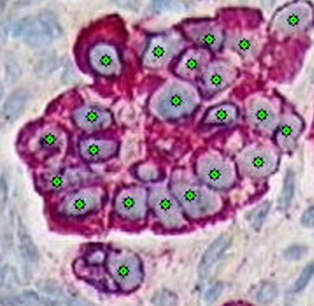
\includegraphics[width=3in]{cancer.png}
\end{figure}

All cells are stained using immunohistochemistry using a compound which appears blue. But cancer cells in this type of immunohistochemical staining appear to have a red membrane due to a surface marker. (In the example above a green dot is placed in the center of every cancer cell to indicate to you what you are looking for; this dot is \emph{not part of the original image}). Assume we are using a data-driven approach to solve this problem.
}

\begin{enumerate}

\easysubproblem{What type of AI would work the best here? No need to discuss.}\spc{1}

\easysubproblem{What is the raw data representation?}\spc{2}

\intermediatesubproblem{What is the unit of analysis?}\spc{3}

\intermediatesubproblem{Why is it easy for you to find the cell centers but difficult for a computer?}\spc{3}

\hardsubproblem{Consider the situation where you employ classic machine learning. What features would you collect on the units of analysis? Enumerate and describe these features.}\spc{8}

\hardsubproblem{How would you sample to build a dataframe (collect historical data)? Explain the procedure and the goals of this step. This is known as \qu{supervised machine learning}.}\spc{7}

\intermediatesubproblem{Once you built the dataframe, would a human be able to use that dataframe to create a predictive model? Yes / no and discuss.}\spc{3}

\easysubproblem{Considering you selected features in (e) and sampled in (f), would this entire enterprise be considered \qu{good machine learning}? Explain.}\spc{3}


\easysubproblem{Now you have the dataframe. Given the problem context, which worldview would you select --- the parametric or the nonparametric and why?}\spc{3}

\hardsubproblem{Assume you went the parametric model route and you built a linear model. Explain where it would be wrong. Be explicit by referencing your predictors in (e).}\spc{10}


\end{enumerate}

\problem{These exercises will dicsuss the linear model and linear regressions.}


\begin{enumerate}

\easysubproblem{Think of three loss functions $L(e_1, \ldots, e_n)$. Do not list any that we did in class.}\spc{3}

\intermediatesubproblem{You are building a data-driven model and choose to use the linear parametric assumption but not necessarily the other three OLS assumptions. Describe a situation where fitting this model using $L = SSE$ is \emph{not} a good idea because it does not accuractely reflect the loss function in your situation at hand.}\spc{3}

\extracreditsubproblem{Prove that the MLE of the $\beta$'s is the same solution as minimizing SSE.}\spc{10}


\extracreditsubproblem{Assume that you have proven the above and plugged in those estimates to the likelihood expression. Now $\sum_{i=1}^n \errorrv_i^2 = \sum_{i=1}^n e_i^2 = SSE$. Prove that $\hat{\sigsq}_{MLE} = MSE$.}\spc{8}



\end{enumerate}

\problem{We will now analyze the baseball data (\texttt{baseball.csv}). You can use any software package you wish to answer these questions.}

\begin{enumerate}

\easysubproblem{Fit a linear model with reponse variable $y:$ salary in thousands. Use all available predictors. Provide a valid interpretation on $\betahat_j$ for the feature \qu{number of RBI's}.}\spc{3}

\easysubproblem{Is this interpretation reasonable given what you know about number of RBI's and how it is related to other predictors? You may need to ask someone who knows a bit about baseball.}\spc{6}

\easysubproblem{What a causal additive model for number of RBI's make sense? Yes / no.}\spc{1}

\easysubproblem{Would you be able to make a randomized experiment to find the additive causal effect of number of RBI's? Yes / no.}\spc{1}

\easysubproblem{Some of these variables may be significant because we dredged. Why is this likely \emph{not} the case?}\spc{3}

\extracreditsubproblem{Use a likelihood ratio test to test the effect of number of RBI's and Number of Walks.}\spc{10}



\end{enumerate}




\end{document}
